\documentclass[a4paper,12pt,leqno]{article}
\usepackage[utf8]{inputenc}
\usepackage[T1]{fontenc}
\usepackage[polish]{babel}
\usepackage{amsmath}
\usepackage{a4wide}
\usepackage{graphicx}
\usepackage{subfig}
\usepackage{wrapfig}

\title{\textbf{Algorytmy ewolucyjne}\\
       {\Large Raport z zadania pierwszego}\\[-1ex]}
\author{Karol Konaszyński i Wiktor Janas}
\date{Wrocław, dnia \today\ r.}

\begin{document}
\maketitle

Niniejszy projekt jest kontynuacją pracy dotyczącej rozpoznawania obrazów. Wówczas udało nam się osiągnąć dobre wyniki, jeśli chodzi o odróżnianie figur geometrycznych i cyfr, a także bardziej
skomplikowanych obrazków, takich jak krótkie słowa i owoce. Wadą dotychczasowego algorytmu był przede wszystkim znaczny czas działania.

Ten projekt rozszerza dotychczasowe podejście w dwóch kierunkach. Po pierwsze, postanowiliśmy przyspieszyć program tak, aby osiągnąć wydajność dającą nadzieje na zastosowania praktyczne.
Po drugie, staraliśmy się uogólnić algorytm tak, aby był zdolny do rozpoznawania fragmentów obrazów, czyli znajdowania znanych obiektów z bazy na mozaikach.

W wyniku realizacji projektu powstały dwa programy. Jeden jest ograniczony do rozpoznawania pojedyńczych obrazów tak, jak było to w poprzedniej części projektu, zawiera jednak znaczne
usprawnienia wydajnościowe. Drugi program jest rozszerzony o rozpoznawanie mozaik, kosztem istotnie większego czasu działania.

\section{Wyszukiwania najbliższych punktów}

Głównym kosztem obliczeniowym algorytmu jest ewaluacja osobników. W celu jej przyspieszenia zastosowano kilka rozwiązań, na przykład podzielono pracę na wątki, aby w pełni wykorzystać 
moc obliczeniową procesora. Jako, że ewaluacja każdego osobnika jest niezależnym zadaniem, w celu uzyskania dalszych przyspieszeń można zastosować procesory masowo równoległe, takie
jak procesory graficzne. 

Ewaluacja pojedyńczego osobnika polega, w uproszczeniu, na zadawaniu znacznej ilości pytań postaci ,,jaki punkt w zbiorze $X$ jest najbliższy punktowi $p$''. Kluczową obserwacją okazało
się, że zbiór $X$ można uczynić stałym (w poprzednim programie zbiór ten był zmienny). W związku z tym przed uruchomieniem właściwej części algorytmu można zastosować preprocessing,
który następnie umożliwi nam natychmiastowe odpowiadanie na pytania. 

Dla ustalonego zbioru $X$ można wyobrazić sobie podział płaszczyzny na fragmenty: każdy fragment $s$ przypisany jest do pewnego punktu $x$ z $X$ w ten sposób, że dla każdego punktu
z $s$ najbliższym punktem z $X$ jest właśnie $x$. Okazuje się, że taki podział płaszczyzny na fragmenty istnieje i nazywa się diagramem Voronoia. Diagram Voronoia dla danego zbioru
$X$ można obliczyć w czasie $n \log n$, gdzie $n = |X|$, jednak jest to zadanie niebanalne; używanie tak uzyskanej struktury również nie byłoby proste. W związku z tym zdecydowaliśmy
się na uproszczone rozwiązanie.

Wyobraźmy sobie, że umieszczamy punkty z $X$ na dwuwymiarowym obrazku oraz, że chcemy dla każdego piksela tego obrazka znaleźć najbliższy mu punkt z $X$. Tak postawiony problem jest
bardzo podobny do powyższego, jednak daje się rozwiązać nieporównywalnie prostszymi metodami: dzięki zastąpieniu matematycznego pojęcia płaszczyzny prostszym pojęciem obrazka, obliczamy
jedynie odległość dla pikseli. Ponadto, możemy dla każdego piksela znaleźć nie jeden najbliższy punkt z $X$, lecz kilka takich punktów, w kolejności rosnącej odległości. Informacja taka
jest wielce użyteczna we właściwej części algorytmu.

Zastosowany algorytm opiera się na algorytmie Dijkstry. Traktujemy obrazek jako graf ważony, a punkty z $X$ jako źródła, dla których odległość wynosi $0$. Uruchamiając algorytm Dijkstry
otrzymujemy rozszerzające się ,,plamy'', które wreszcie pokrywają cały obrazek. Pamiętając, w jakiej kolejności dany piksel był zalewany (tzn. która plama dotarła do niego pierwsza, która
druga itd) otrzymujemy dla owego piksela kolejne najbliższe mu punkty z $X$. Obliczenia te nie są szybkie, jednak trwają też bardzo długo; wynik jest zapamiętywany podobnie jak wynik
wyszukiwania punktów charakterystycznych. Dzięki temu dla danego obrazka program wykonuje obliczenia jedynie raz, przy następnych uruchomieniach korzysta z wcześniej obliczonych danych.

Przedstawione podejście może nasuwać dwa pytania. Po pierwsze, co, jeżeli chcemy znać najbliższy punkt dla punktu, którego współrzędne nie są całkowite (jest to normalne zjawisko, gdyż
punkty, o które pytamy są punktami charakterystcznymi przemnożonymi przez macierz, której współczynniki nie muszą być całkowite). Prostym rozwiązaniem tej kwestii jest zaokrąglenie
współrzędnych. Okazuje się, że nie jest to zły pomysł, gdyż w większości wypadków pytanie o punkt wypada w środku ,,plamy'' i dla wszystkich punktów w otoczeniu odpowiedź jest taka sama.
Warto również zastanowić się, jakiej odpowiedzi udzielimy dla punktów, które znajdują się na styku plam. Łatwo zauważyć, że punkty takie znajdują się w podobnej odległości od obu źródeł,
więc nawet jeżeli nie udzielimy dokładnej odpowiedzi (bo współrzędne zaokrąglą się ,,nie w tą stronę''), to popełniany błąd będzie bardzo niewielki. Istotnie, eksperymenty wykazały, że
odległość liczona metodą brutalną może różnić się od odległości wziętej z mapy o conajwyżej ułamki procenta.

Przykładową mapę pobliskich punktów prezentuje rysunek \ref{proxmap}. Przedstawiono na nim obrazek wyjściowy, znalezione punkty charakterystyczne, najbliższe punkty oraz drugie najbliższe
punkty. Wizualizacja najbliższych punktów opiera się na naiwnym algorytmie kolorowania grafu planarnego, zatem można być prawie pewnym, że sąsiadujące ze sobą obszary są zaznaczone
różnymi kolorami. Warto zwrócić uwagę, że sturuktura drugich najbliższych punktów jest bardzo skomplikowana. Koszt obliczenia takiej mapy to około rozmiar obrazka razy ilość najbliższych
punktów, które chcemy spamiętać dla każdego piksela. W przedstawionym przykładzie jest to $400 \times 322 \times 6 \approx 0.7 \text{mln}$. Obliczenia takie trwają kilka sekund. Algorytm 
obliczania tej mapy nie został zrównoleglony, zatem wykorzystuje tylko jeden rdzeń procesora. Zrównoleglenie algorytmu prawdopodobnie jest możliwe, ale nie wydaje się proste.

\begin{figure}\centering
\subfloat[obrazek + poi]{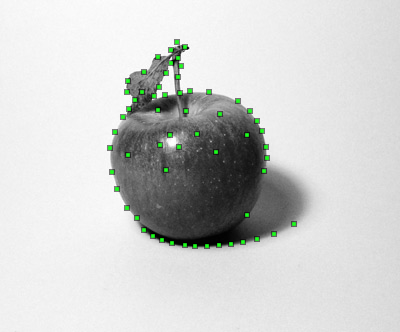
\includegraphics[width=5cm,keepaspectratio=true]{./proxmap/apple-pois.png}}\hspace{1mm}
\subfloat[najbliższe punkty]{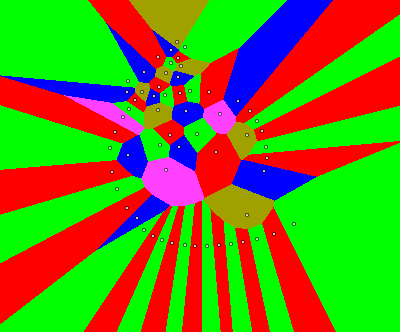
\includegraphics[width=5cm,keepaspectratio=true]{./proxmap/apple-prox-0.png}}\hspace{1mm}
\subfloat[drugie najbliższe punkty]{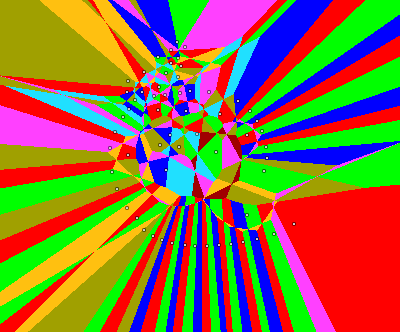
\includegraphics[width=5cm,keepaspectratio=true]{./proxmap/apple-prox-1.png}}\hspace{1mm}
\caption{Mapa pobliskich punktów}{\label{proxmap}}
\end{figure}

\section{Zmienne parametry ewolucji}

Analizując wpływ parametrów na działanie poprzedniego programu zauważyliśmy, że bardzo istotna jest wartość współczynnika przetrwania. Mianowicie, niskie współczynniki przetrwania
powodują bardzo szybką zbieżność populacji. Jest to efekt pożądany w momencie, gdy algorytm jest już blisko rozwiązania optymalnego: umożliwia bowiem skoncentrowanie wszystkich
osobników na optymalizacji tego właśnie rozwiązania. Z drugiej strony nie można prowadzić ewolucji od początku z niskim współczynnikiem przetrwania, gdyż spowoduje to szybką
zbieżność do ,,pierwszego lepszego'' minimum.

W związku z powyższą obserwacją, wprowadziliśmy do algorytmu zmienny współczynnik przetrwania. Jego wartość jest opisana wielomianem, którego argumentem jest liczba z zakresu
$0 \dots 1$, przy czym $0$ oznacza pierwsze, a $1$ ostatnie pokolenie ewolucji (ilość pokoleń jest z góry ustalona). Wielomian ten jest dany w pliku konfiguracyjnym i dla programu
rozpoznającego pojedyńcze obrazki ma postać $-0.3x + 0.8$, zaś dla programu pracującego z mozaikami $-0.2 + 0.8$. Oznacza to, że wartość współczynnika przetrwania zmienia się
liniowo od $80\%$ do $50\%$ lub $60\%$. Przeprowadziliśmy eksperymenty z wielomianami wyższego stopnia, jednak nie okazały się one wyraźnie lepsze. Obserwując działanie programu
wyraźnie widać, jak malejący współczynnik przetrwania (widoczny w pasku na dole) ,,ogniskuje'' populacje.

W przypadku programu rozpoznającego mozaiki poszliśmy krok dalej: wprowadziliśmy również zmienne wspólczynniki mutacji. Zadanie tego programu jest istotnie różne od programu
rozpoznającego pojedyńcze obrazy. Najpierw chcemy starannie przeszukać całą przestrzeń rozwiązań, aby znaleźć ,,ogniska'', to znaczy miejsca, w których znajdują się pod-obrazy mozaiki.
Następnie chcemy koncentrować się na optymalizacji w tych obszarach. Dlatego też na początku współczynniki mutacji są zwiększone, później zaś maleją. Wprowadzenie tej zmiany istotnie
poprawiło wyniki osiągane przez program.

\section{Prace nad mozaikami}

Przez \textit{mozaikę} rozumiemy obrazek będący sklejeniem kilku (najczęściej czterech) obrazów podstawowych.
Naszym celem jest rozpoznanie obrazków składowych takiej mozaiki, czyli dopasowanie obrazków z bazy danych do fragmentu zapytania.
Niestety, algorytm badany w pierwszej części projektu nie działał dla takich testów.

\subsection{Gęstość zbioru POI}
Podstawowym problemem, jaki musieliśmy rozwiązać, jest skalowanie zbioru punktów charakterystycznych. 
Poprzednio bowiem rozmiar tego zbioru wybierany był ,,na sztywno'', przed wykonaniem jakichkolwiek przekształceń. Niestety, skutkiem tego była niewspółmierna gęstość POI. Jako, że mozaika
zawiera cztery obrazy, zawiera również cztery razy więcej szczegółów, czyli punktów charakterystycznych. Ustalenie rozmiaru zbioru POI na sztywno powodowało, że POI mozaiki
były rozmieszczone dużo rzadziej, niż POI obrazu z bazy. Jednocześnie osobniki, które starają się dopasować obraz z bazy poprzez zmniejszenie go, bardzo mocno zagęszczają POI.
Co gorsza, efekty te kumulują się: rozrzedzenie POI zapytania i zagęszczenie POI obrazka z bazy powoduje, że dopasowanie obrazów nastręcza znaczne trudności.

Zastosowane rozwiązanie wydaje się być dość naturalne. Zmodyfikowaliśmy algorytm wyszukiwania punktów charakterystycznych tak, aby najpierw wyszukiwał pewną z góry zadaną ilość POI na 
obrazku z zapytania; następnie dla przekształconych obrazów z bazy odpowiadających poszczególnym osobnikiom wybieramy zbiór POI tak, aby ich gęstość była podobna do gęstości punktów w 
zapytaniu. Niestety, algorytm wyszukujący punkty charakterystyczne na obrazie jest mało wydajny. Na szczęście działa on w dwóch fazach. Główny koszt obliczeniowy wiąże się z 
określeniem ,,ciekawości'' każdego piksela. Następnie względnie szybko daje się wybrać pewną ilość najlepszych pikseli, dbając o to, aby nie były one zbyt blisko siebie (parametr decydujący o
dopuszczalnej gęstości POI nazywa się \textit{tabu}). Po modyfikacjach algorytm działa następująco:
\begin{enumerate}
 \item oblicz ,,ciekawość'' dla każdego piksela obrazka z zapytania oraz wybierz wiele (około tysiąca) najciekawszych punktów.
 \item przefiltruj wybrane punkty tak, aby pozostała ich rozsądna ilość (80 -- 150).
 \item oblicz ,,ciekawość'' dla każdego piksela obrazka z bazy oraz wybierz wiele (około tysiąca) najciekawszych punktów.
 \item podczas ewaluacji osobnika, przekształć punkty wybrane w kroku 3 używając macierzy osobnika;
       następnie z otrzymanego zbioru wybierz punkty tak, aby ich gęstość odpowiadała gęstości punktów wybranych w kroku 2
\end{enumerate}

Powyższe rozwiązanie okazało się mieć wady i zalety. Podstawową wadą jest trywialne maksimum globalne funkcji celu. Jeżeli bowiem ściśnie się obrazek z bazy danych, wszystkie punkty wybrane
w kroku 3 przejdą na bardzo niewielki obszar; następnie filtrowanie z kroku 4 pozostawi jeden lub dwa punkty. W takim przypadku wystarczy, że punkty te znajdą się niedaleko jakiegokolwiek
POI zapytania. Efekt ten zmusił skłonił nas do sformułowania bardziej wyrafinowanego pojęcia ,,podobieństwa''. 

\subsection{Analiza podobieństwa obrazków}
Dwa obrazki $O_1$, $O_2$ są podobne, jeżeli istnieje przekształcenie afiniczne $F$, dla którego odległość POI obrazków $O_1$, $F(O_2)$ jest relatywnie mała.
Ponadto wymagamy, aby $F$ oraz $F^{-1}$ skalowały co najwyżej czterokrotnie oraz ściskały conajwyżej dwukrotnie, gdzie skalowanie definiujemy jako
\[ s_f = \max_{\vec x \in R^2} \| f(\vec x) \| / \| \vec x \| \]
zaś ściskanie jako
\[ c_f = \max_{\vec x, \vec y \in R^2, \vec x \bot \vec y} \| f(\vec x) \| / \| f(\vec y) \| \]

W powyższej definicji należy jeszcze uściślić pojęcie odległości POI dwóch obrazków. Pamiętając o tym, że traktujemy POI obrazka jako zbiór (równorzędnych) punktów, 
musimy określić (asymetryczną) funkcję odległości jednego zbioru punktów od drugiego. W dalszym ciągu umawiamy się, że liczymy odległość punktów z obrazka bazowego do obrazka z zapytania.
Do tej pory ogólnym schematem było znalezienie dla każdego punktu z przekształconego obrazka z bazy najbliższego mu punktu w zapytaniu, a następnie policzenie odległości między nimi.
Odległość zbiorów definiowana była jako średnią powyższych odległości. Okazuje się jednak, że takie proste podejście jest niewystarczające.

\paragraph{Przeszkoda 1: wiele do jednego}
Ponieważ punkty mają ustaloną gęstość, od ,,bliskich'' sobie obrazków oczekujemy, by ich punkty dopasowywały się ,,1-1''. 
Chcielibyśmy wyeliminować sytuacje, w których do jednego punktu z zapytania dopasowywanych było wiele punktów z obrazka bazowego.
W pierwotnym programie problem ten rozwiązywany był poprzez liczenie odległości od zapytania do obrazka z bazy oraz od obrazka z bazy do zapytania.
Podejście to jednak nie ma zastosowania w obecnym projekcie, gdzie do wyszukiwania najbliższych punktów zastosowano diagram Voronoia. Obliczanie tej struktury
jest kosztowne czasowo, zatem można sobie na to pozwolić jedynie w przypadku obrazka z zapytania, jako że nie ulega on zmianom w czasie. Brak owej struktury dla
przekształconego obrazka z bazy eliminuje możliwość obliczania odległości z zapytania do obrazka z bazy. Ponadto w programie rozpoznającym fragmenty mozaik liczenie
owej odległości jest wręcz niemożliwe: celowe jest, aby część punktów z zapytania pozostała niedopasowana, zatem należy się spodziewać wielkich odległości z tych
punktów do punktów przekształconego obrazka z bazy.

Odległość między obrazkami jest przeto obliczana jedynie z obrazka z bazy do obrazka z zapytania. Dobrym rozwiązaniem powyższych trudności okazało się zliczanie,
ile punktów z obrazka bazowego wskazało jako swojego najbliższego sąsiada dany punkt z zapytania.

W programie rozpoznającym pojedyńcze obrazki wprowadzono następnie ograniczenie na maksymalną ilość takich wskazań: mianowicie punkt z zapytania może zostać
wskazany przez conajwyżej dwa punkty obrazka z bazy. Jeżeli dla punktu z obrazka bazowego najbliższy znaleziony punkt z zapytania jest już zajęty (został
wykorzystany dwa razy), znajdowany jest drugi co do odległości punkt, jeżeli on też jest zajęty, znajdowany jest trzeci i tak dalej aż do szóstego. Jeżeli
żaden z sześciu najbliższych punktów nie jest wolny, punkt z obrazka bazowego pozostaje niedopasowany i osobnikowi przydzielana jest zaporowa kara.

W programie rozpoznającym mozaiki badany jest zbiór liczb naturalnych oznaczających ilość dopasowań do każdego z punktów z zapytania. Obliczana jest średnia
$W$ niezerowych elementów tego zbioru. Następnie średnia obliczona średnia odległość mnożona jest odległość przez $e^{W-1}$. W ten sposób karane są
osobniki próbujące dopasować kilka swoich POI do jednego.

\paragraph{Przeszkoda 2: małe jest lepsze}
Dość intuicyjnym faktem jest to, że osobniki, których przekształcenie mocniej ściska obrazek, okazują się być średnio lepsze. Wynika to stąd, że dopasowanie opiera
się jedynie na punktach charakterystycznych; im mniejszy obrazek, tym mniej owych punktów, a zatem łatwiej wskazać jakikolwiek fragment zapytania, w którym punkty
rozkładają się podobnie. Ekstremalnym przypadkiem tego problemu jest ściśnięcie obrazka tak bardzo, że zostaje z niego tylko jeden punkt. Oczywiście dopasowanie
pojedyńczego punktu nie nastręcza żadnych trudności niezależnie od tego, co znajduje się na obrazku z zapytania. Należy zauważyć, że problem ten występuje jedynie
w programie rozpoznającym mozaiki. Program dopasowujący pojedyńcze obrazki nie próbuje kompensować zmian gęstości POI, zatem próby drastycznego zmniejszenia obrazka
powodują powstanie ogromnego zagęszczenia POI, które nie daje się dobrze dopasować według reguł opisanych powyżej lub otrzymuje wielkie kary z względów opisanych poniżej.

Zastosowane rozwiązanie polega na wprowadzeniu do funkcji celu ,,rozpiętości'' obrazka. Dzieląc wartość funkcji celu przez ,,rozpiętość'' przekształconego obrazka z 
bazy promujemy większe osobniki, a udzielamy kary mniejszym. Ponieważ zastosowane rozwiązanie jest całkowitą heurystyką, ,,rozpiętość'' zdefiniowano jako długość
przekątnej prostokąta zawierającego wszystkie przekształcone punkty obrazka bazowego. Prawdopodobnie lepszą miarą byłby promień najmniejszego koła pokrywającego,
lecz obliczenie tej wielkości jest niebanalne.

\paragraph{Przeszkoda 3: bagatelizacja małych błędów}
Okazuje się, że nawet w przypadku nawet niemal identycznych obrazków ich POI nie będą idealnie się pokrywały. Wynika to między innymi ze specyfiki algorytmu oceny
,,ciekawości'' pikseli, który nie jest niezmienniczy względem obrotów i skalowań, jak również ze znacznych trudności z znalezieniem perfekcyjnego dopasowania przy
użyciu algorytmów ewolucyjnych. Chcemy zatem nazwać dopasowanie dobrym, jeżeli odległość między POI z bazy, a POI z zapytania jest rzędu wielkości średniej odległości
POI w zapytaniu. Można to sobie wyobrazić w następujący sposób: rozpatrzmy obraz z ostrą krawędzią. Punkty charakterystyczne na owej krawędzi rozmieszczone będą
dość równomiernie (aby to sprawdzić, wystarczy uruchomić któryś z przykładów geometrycznych lub tekstowych). Nie musimy wymagać, aby punkty z bazy pokryły się idealnie
z punktami z zapytania; wystarczy nam jedynie, aby między każdymi dwoma punktami z zapytania znalazł się jakiś punkt z bazy (czyli, aby punkty z bazy również były
rozmieszczone równomiernie wzdłuż rozpatrywanej krawędzi).

Aby osiągnąć ten efekt, wprowadzamy nieliniową funkcję odległości POI. Najpierw obliczamy średnią odległość między punktami charakterystycznymi z zapytania (wystarczy
zrobić to raz, gdyż obrazek z zapytania nie zmienia sie). Następnie, jeżeli znaleziona odległość POI bazowego od najbliższego mu POI z zapytania nie przekracza połowy
owej średniej odległości, funkcja jest liniowa, jeżeli zaś przekracza -- sześcienna. Formalniej, niech $\mathrm{avg}_t$ będzie średnią odległością między POI obrazka
z zapytania, zaś $d$ odległością euklidesową rozpatrywanych POI. Wówczas odległość użyta do obliczania funkcji celu wyraża się wzorem:
\[ d' = \begin{cases}
	    d & \text{jeżeli } d < \mathrm{avg}_t / 2 \\
	    d^3 / 4\mathrm{avg}_t^2 & \text{w przeciwnym wypadku}
	 \end{cases} \]
Współczynnik $1 / 4\mathrm{avg}_t^2$ zapewnia ciągłość funkcji w punkcie $d$.

\paragraph{Przeszkoda 4: wszechstronne kształty}
Problem ten jest głównym mankamentem algorytmu. Okazuje się, że istnieją kształty podobne do wielu kształtów jednocześnie. Przykładowo ogonek wisienki jest podobny do
krawędzi banana, zaś jej ciało dobrze dopasuje się na przykład do pomarańczy. Okazuje się, że nietrywialne kształty często ściągają do siebie bardzo wiele dopasowań;
nawet jeżeli nie są to dopasowania bardzo dobre, to algorytm znajduje je, gdyż są proste.
Pojawiło się kilka pomysłów na wyeliminowanie tego problemu. Najbardziej obiecującym z nich był powrót do koncepcji symetrycznej odległości, czyli sumy odległości z obrazka bazowego
do zapytania i odwrotnie. Oczywiście ze względu na opisane wcześniej komplikacje, wymagane byłyby zmiany; możnaby na przykład dopasowywać cały obrazek bazowy do tego fragmentu obrazka
z zapytania, który leży bezpośrednio pod nim. Innym podejściem byłoby dodanie do osobnika maski bitowej oznaczającej, które punkty z zapytania staramy się dopasować. W przypadku prostych
mozaik możnaby wręcz zastosować osobny algorytm do podzielenia obrazu na części, a następnie dla każdej z znalezionych części uruchomić algorytm dopasowujący pojedyńcze obrazki.
Sprawdziliśmy kilka obiecująco brzmiących rozwiązań, jednak żadne z nich nie sprawdziło się w praktyce. Na szczęście problem ten nie manifestuje się w przypadku prostych testów.

\section{Testy moizaikowe}

Dzięki powyższym modyfikacjom udało się zmusić algorytm do działania na niektórych, prostszych, mozaikach. Dobrze działają mozaiki złożone z prostych figur geometrycznych,
jednakże z bardziej skomplikowanymi kształtami program sobie nie radzi. W szczególności niewypałem okazały się próby użycia go do mozaik owocowych, czy zawierających cyfry.
Poniżej przedstawiamy wykonane testy.

\subsection{Testy geometryczne}

\paragraph{Test pierwszy: okrąg, kwadrat, trójkąt, krzyż}
W tym teście mozaika składa się z czterech powyżej wymienionych figur. Jest to test najprostszy, gdyż figury mają prosty oraz istotnie różny kształt. Okazuje się, że algorytm sprawdza
się prawie idealnie (myli się tylko się raz na kilka uruchomień). Rezultaty działania oceniamy wyłącznie intuicyjnie, starając się określić, czy algorytm znalazł wystarczająco
dobre dopasowanie. Wyniki liczbowe są następujące: 
\begin{verbatim}
geom/square.png: -0.484211
geom/cross.png: -2.293484
geom/circle.png: -3.587710
geom/house.png: -3.607674
geom/clover.png: -4.487347
geom/triangle1.png: -5.323895
geom/balls.png: -13.413114
geom/4star.png: -26.052204
geom/arch.png: -30.556473
geom/5star.png: -37.949917
\end{verbatim}
Rysunki \ref{test1-pics} pokazują, że istotnie program skutecznie rozpoznaje znane obrazy oraz poprawnie znajduje dopasowania obrazów ,,podobnych''. Kwadrat poprawnie dopasował się
do kwadratu, okrąg niestety także do kwadratu, wynika to z (zamierzonej) niedoskonałości obu rysunków. Podobnie niewielką odległość okazały się mieć krzyż oraz czterolistna koniczyna
(zgodnie z oczekiwaniami) oraz trójkąt i ,,domek'' (podobny do trójkąta). Pozostałe figury mają niską funkcję celu, zatem możemy stwierdzić, że program (poprawnie) nie odnalazł ich
na mozaice.

\begin{figure}\centering
\subfloat[kwadrat]{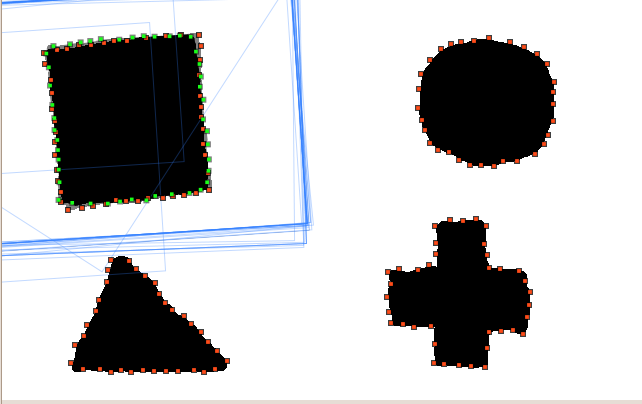
\includegraphics[width=5cm,keepaspectratio=true]{./test1/match1.png}}\hspace{1mm}
\subfloat[krzyż]{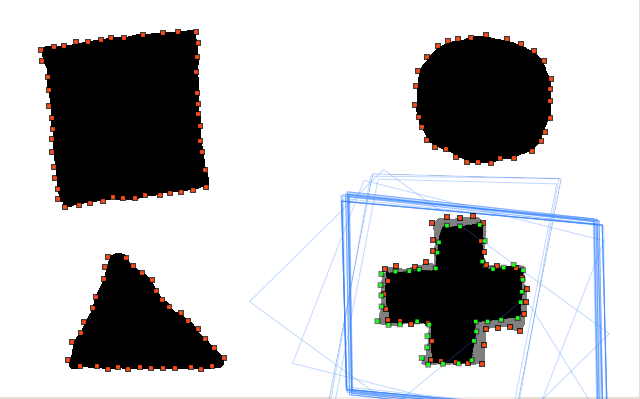
\includegraphics[width=5cm,keepaspectratio=true]{./test1/match2.png}}\hspace{1mm}
\subfloat[koło]{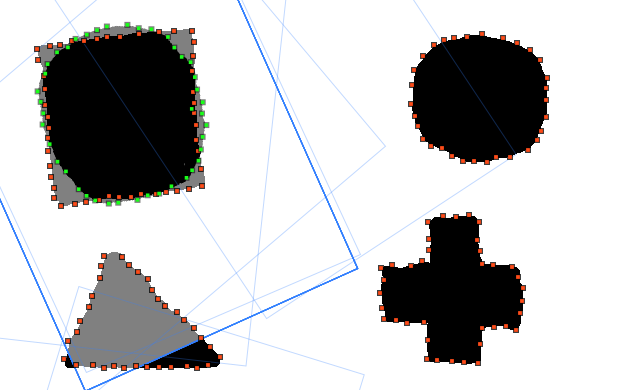
\includegraphics[width=5cm,keepaspectratio=true]{./test1/match3.png}}\hspace{1mm}
\subfloat[trójkąt]{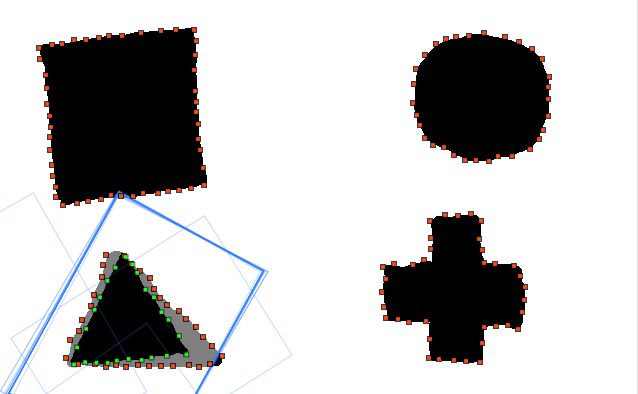
\includegraphics[width=5cm,keepaspectratio=true]{./test1/match4.png}}\hspace{1mm}
\subfloat[gwiazda 5-cio ramienna]{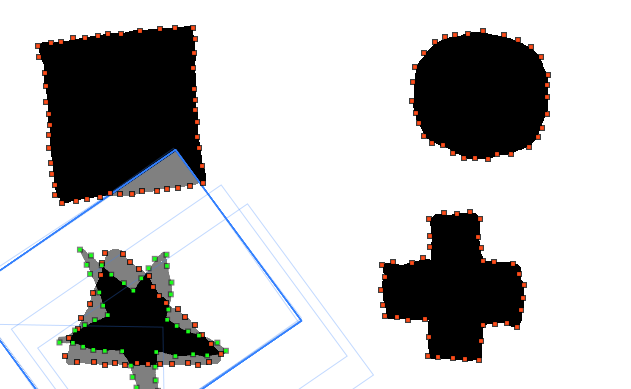
\includegraphics[width=5cm,keepaspectratio=true]{./test1/match5.png}}\hspace{1mm}
\subfloat[gwiazda 4-ro ramienna]{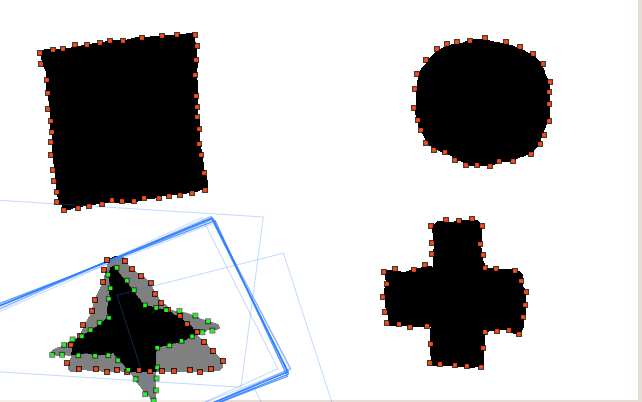
\includegraphics[width=5cm,keepaspectratio=true]{./test1/match6.png}}\hspace{1mm}
\subfloat[dwa koła]{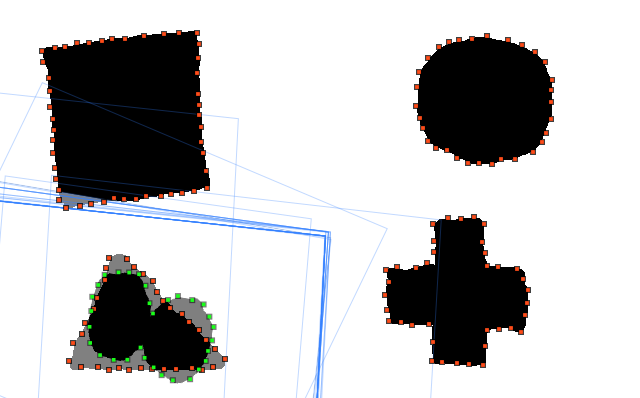
\includegraphics[width=5cm,keepaspectratio=true]{./test1/match7.png}}\hspace{1mm}
\subfloat[podkowa]{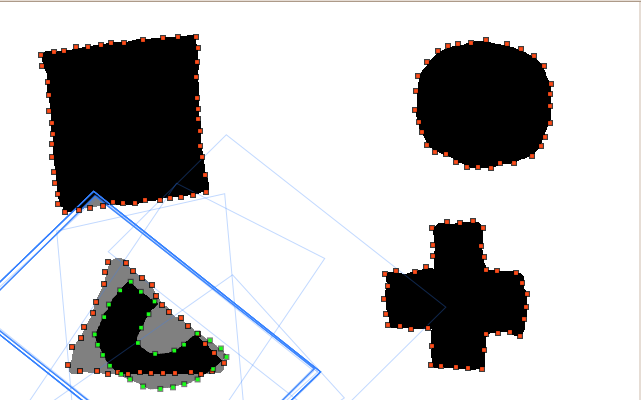
\includegraphics[width=5cm,keepaspectratio=true]{./test1/match8.png}}\hspace{1mm}
\subfloat[4-ro listna koniczyna]{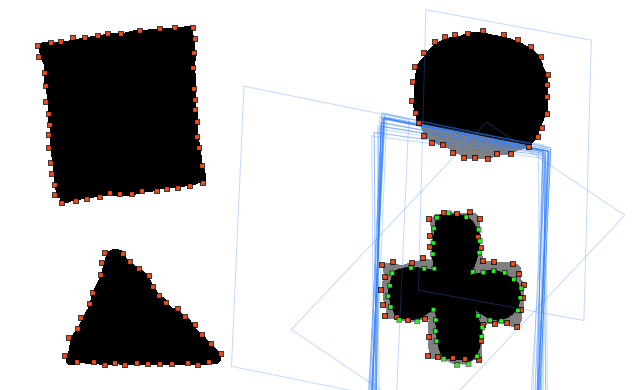
\includegraphics[width=5cm,keepaspectratio=true]{./test1/match9.png}}\hspace{1mm}
\subfloat[domek]{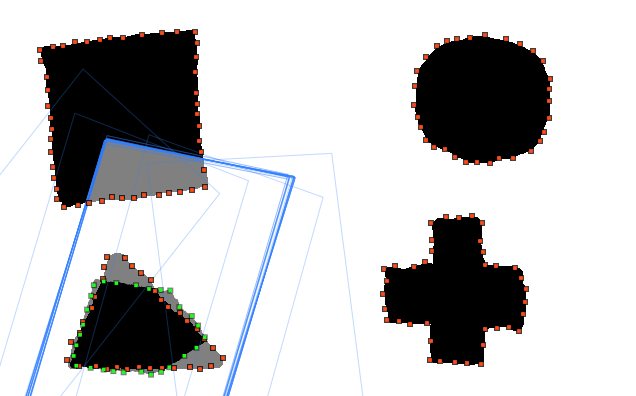
\includegraphics[width=5cm,keepaspectratio=true]{./test1/match10.png}}\hspace{1mm}
\caption{Dopasowania figur do mozaiki, test 1}{\label{test1-pics}}
\end{figure}

\paragraph{Test drugi: uśmiech, domek, koniczyna, muszka}
W tym teście postanowiliśmy zrobić mozaikę z bardziej skomplikowanych figur. Wyniki nadal są zadowalające, jednak częściej zdarzają się błedy.
Oto wynik typowego uruchomienia:
\begin{verbatim}
geom/triangle1.png: -1.089741
geom/clover.png: -2.495673
geom/balls.png: -2.622310
geom/circle.png: -2.776270
geom/house.png: -2.873120
geom/square.png: -3.610290
geom/cross.png: -4.051198
geom/arch.png: -5.901488
geom/4star.png: -13.952413
geom/5star.png: -31.386328
\end{verbatim}
Teraz skupimy się na bardziej interesujących dopasowaniach.
Bardzo dobrze odnalazł się trójkąt we fragmencie muszki. Koniczyna dopasowała sie bez zarzutu, do muszki także podobne są dwa złączone kółka.
Natomiast uśmiech okazał się relatywnie podobny do podkowy (łuku). Niestety, nie udało się znaleźć dopasowania domku do domku. 
Ale nie można być idealnym. Na potwierdzenie słów, przedstawiamy kilka rezultatów działania: \ref{test3-pics}.

\begin{figure}\centering
\subfloat[trójkąt]{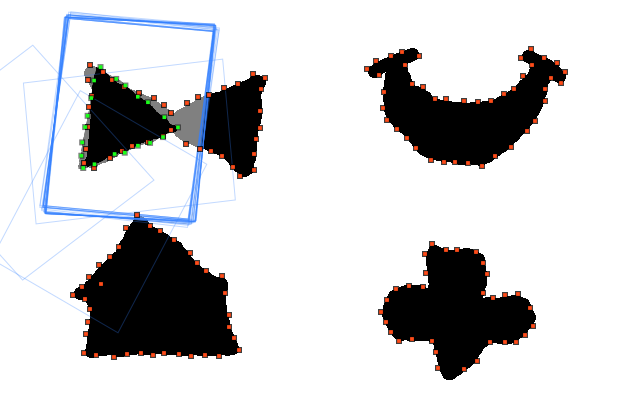
\includegraphics[width=5cm,keepaspectratio=true]{./test3/match4.png}}\hspace{1mm}
\subfloat[podkowa (arch)]{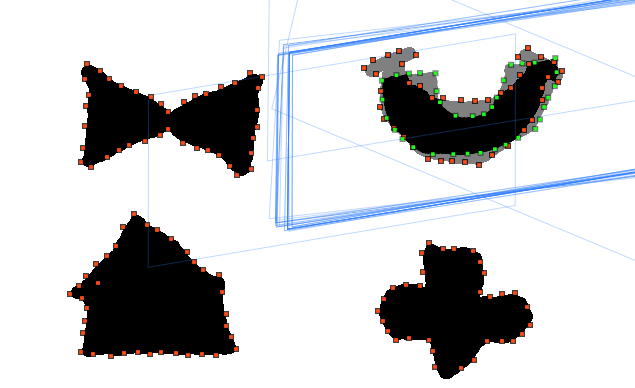
\includegraphics[width=5cm,keepaspectratio=true]{./test3/match8.png}}\hspace{1mm}
\subfloat[kulki]{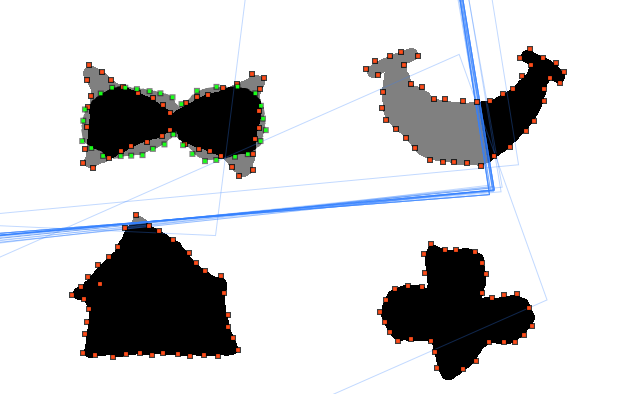
\includegraphics[width=5cm,keepaspectratio=true]{./test3/match7.png}}\hspace{1mm}
\subfloat[domek]{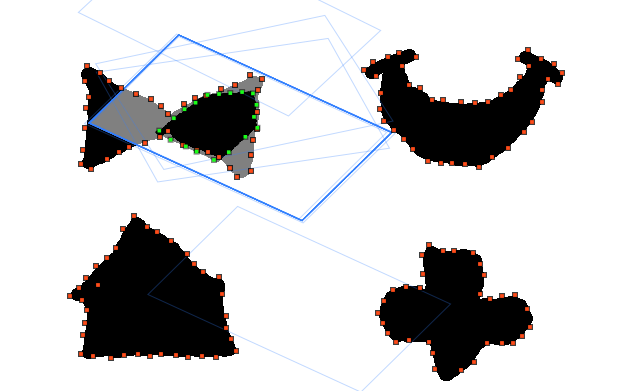
\includegraphics[width=5cm,keepaspectratio=true]{./test3/match10.png}}\hspace{1mm}
\subfloat[gwiazda 5-cio ramienna]{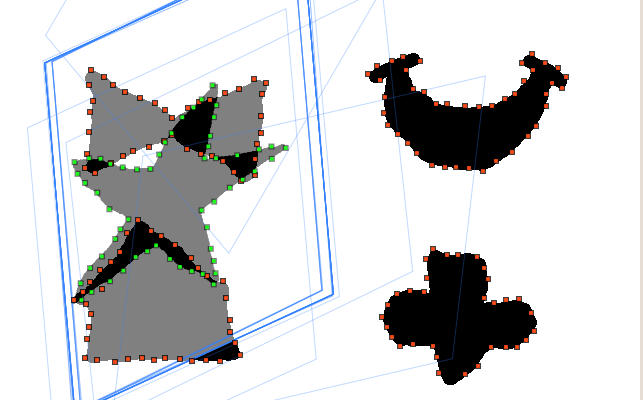
\includegraphics[width=5cm,keepaspectratio=true]{./test3/match5.png}}
\caption{Dopasowania figur do mozaiki, test 2}{\label{test3-pics}}
\end{figure}


Oczywiście, moglibyśmy pokazać więcej chlubnych przykładów działania naszego algorytmu, chcemy jednak zaprezentować testy niedziałające, aby zilustrować przeszkody, które stanęły 
nam na drodze.

\subsection{Testy z cyframi}
\paragraph{Test typowy, ale niedziałający: 2, 3, 6}
W niniejszym teście będziemy starali się rozpoznać co jest na mozaice złożonej z kilku cyfr. Warto wspomnieć, że każdy z elementów mozaiki z osobna dobrze bądź idealnie dopasowuje się do
pewnego obrazka z bazy danych.

Niestety, żadna z cyfr (2,3,6) nie dopasowała się poprawnie do odpowiedniego fragmentu mozaiki. Rezultaty widać na \ref{test5-pics}. Zaś wyniki numeryczne są następujące:
\begin{verbatim}
digs/2_3.pgm: -1.945461
digs/5_3.pgm: -2.889184
digs/1_3.pgm: -2.903626
digs/4_3a.pgm: -3.062191
digs/3_3.pgm: -3.097243
digs/7_3b.pgm: -3.113612
digs/7_3a.pgm: -3.454084
digs/8_3.pgm: -4.048234
digs/9_3.pgm: -4.214192
digs/6_3.pgm: -4.326057
digs/4_3b.pgm: -5.482895
\end{verbatim}
Patrząc na obrazki, można dostrzec 

\begin{figure}\centering
\subfloat[dwójka]{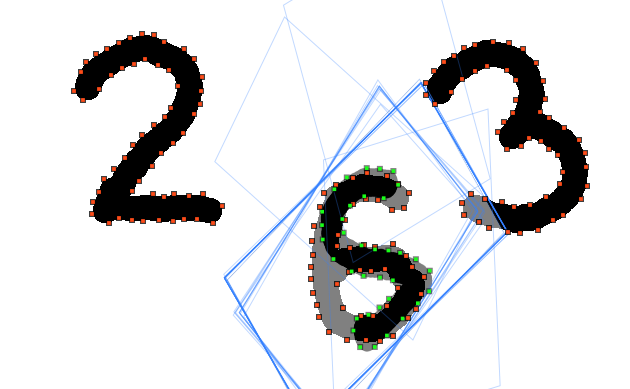
\includegraphics[width=5cm,keepaspectratio=true]{./test5/match2.png}}\hspace{1mm}
\subfloat[trójka{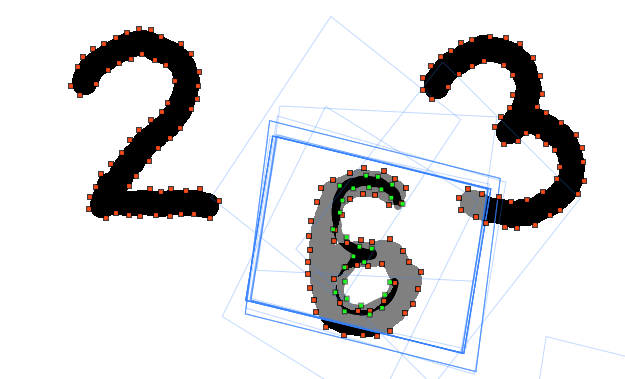
\includegraphics[width=5cm,keepaspectratio=true]{./test5/match3.png}}\hspace{1mm}
\subfloat[czwórka]{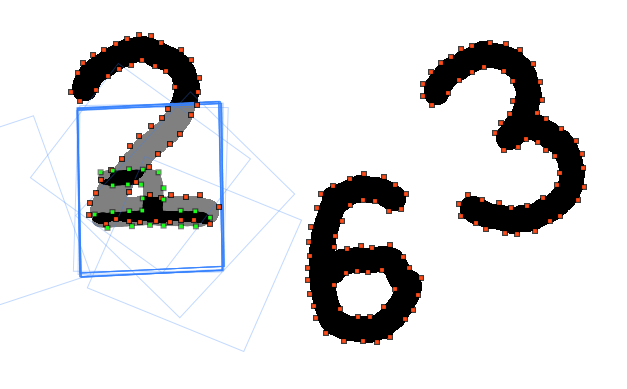
\includegraphics[width=5cm,keepaspectratio=true]{./test5/match5.png}}\hspace{1mm}
\subfloat[szóstka]{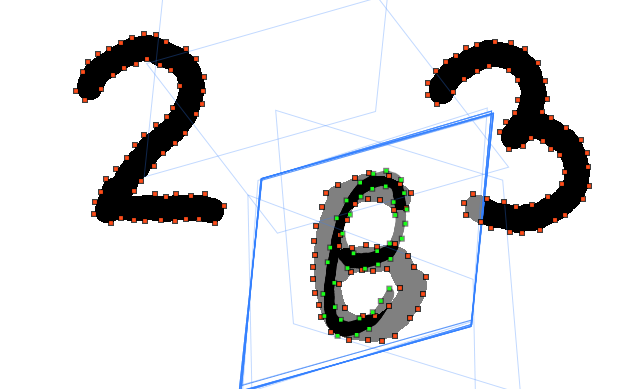
\includegraphics[width=5cm,keepaspectratio=true]{./test5/match7.png}}\hspace{1mm}
\subfloat[dziewiątka]{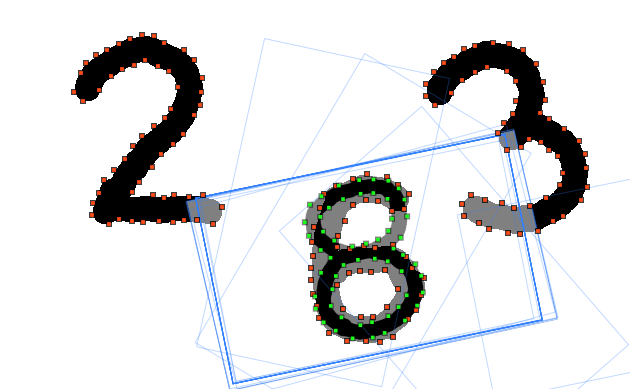
\includegraphics[width=5cm,keepaspectratio=true]{./test5/match10.png}}\hspace{1mm}
\caption{Dopasowania cyfr do mozaiki, test 3}{\label{test5-pics}}
\end{figure}


\section{Uwagi implementacyjne}

Program wymaga systemu operacyjnego GNU/Linux. Do jego kompilacji niezbędne są, poza standardowymi narzędziami, pliki nagłówkowe biblioteki GTK+,
zazwyczaj dostępne w pakiecie \texttt{libgtk2.0-dev} lub podobnym. Aby skompilować program należy w katalogu ze źródłami wydać polecenie \texttt{make}.
W wyniku jego wykonania powinny powstać plii wykonywalne o nazwie \texttt{evolution} oraz \texttt{evosingle}. Programy przyjmują dwa parametry, plik z
obrazkiem-zapytaniem oraz zbiór obrazków z bazy danych. Zbiór ten może zostać podany albo jako kolejne nazwy plików, bądź też jako jedna nazwa pliku
wskazująca na listę plików. Przykładowe wywołania mogą zatem wyglądać następująco:
\begin{verbatim}./evolution geom/square.pgm geom/square2.pgm geom/circle.png
./evolution fruits/apple-mod.pgm db.fruits\end{verbatim}
gdzie plik \texttt{db.fruits} zawiera
\begin{verbatim}
fruits/cherry2.pgm
fruits/cherries.pgm
fruits/banana1.pgm
fruits/apple.pgm
fruits/orange1.pgm
fruits/pineapple.pgm
fruits/watermelon.pgm
fruits/paprika1.pgm
fruits/pear1.pgm
\end{verbatim}
Gdy program otrzymuje obraz do analizy po raz pierwszy, niezbędne jest wyszukanie punktów charakterystycznych oraz zbudowanie mapy pobliskich punktów.
Jest to długotrwała czynność (może trwać nawet pół minuty dla jednego obrazka), wyniki są zapisywane na dysk i przy kolejnych uruchomieniach program
będzie korzystał z obliczonych wcześniej danych. Program wczytuje obrazy w wielu formatach (korzystając z funkcji udostępnianych przez bibliotekę GTK+),
w szczególności dostępne są formaty \texttt{png}, \texttt{jpeg} oraz \texttt{pgm}. Podczas wczytywania obrazów kolorowych, program bierze pod uwagę
\emph{jedynie kanał czerwony}, zatem przed załadowaniem obrazu należy przekonwertować go do skali szarości (ściśle rzecz ujmując, obrazy muszą być zapisane
jako kolorowe, jednak wszystkie składowe koloru powinny być równe). Wraz z kodem źródłowym dostarczane są przykładowe obrazy (w katalogach \texttt{digs},
\texttt{fruits}, \texttt{geom}, \texttt{noise} oraz \texttt{text}). Parametry programu decydujące o działaniu algortymu zostały umieszczone w plikach
\texttt{evolution.cfg} oraz \texttt{evosingle.cfg}, które są wczytywane przez program podczas startu.

Kod źródłowy podzielony jest na kilka plików. Główna część programu znajduje się w pliku \texttt{evolution.C}/\texttt{evosingle.C}. Plik \texttt{poi.C}
zawiera algorytm wyszukiwania punktów charakterystycznych oraz obsługę mapy pobliskich punktów. Plik \texttt{image.c} zawierają kod operacji na obrazkach.
Pliki \texttt{gui.C} oraz \texttt{gui-gtk.c} zawierają implementację graficznego interfejsu użytkownika. Plik \texttt{util.C} zawiera wspólne funkcje takie,
jak operacje na macierzach, punktach, czy framework dla przetwarzania wielowątkowego, zaś plik \texttt{config.C} zawiera parser konfiguracji.

\end{document}
